% Options for packages loaded elsewhere
\PassOptionsToPackage{unicode}{hyperref}
\PassOptionsToPackage{hyphens}{url}
%
\documentclass[
]{book}
\usepackage{amsmath,amssymb}
\usepackage{iftex}
\ifPDFTeX
  \usepackage[T1]{fontenc}
  \usepackage[utf8]{inputenc}
  \usepackage{textcomp} % provide euro and other symbols
\else % if luatex or xetex
  \usepackage{unicode-math} % this also loads fontspec
  \defaultfontfeatures{Scale=MatchLowercase}
  \defaultfontfeatures[\rmfamily]{Ligatures=TeX,Scale=1}
\fi
\usepackage{lmodern}
\ifPDFTeX\else
  % xetex/luatex font selection
\fi
% Use upquote if available, for straight quotes in verbatim environments
\IfFileExists{upquote.sty}{\usepackage{upquote}}{}
\IfFileExists{microtype.sty}{% use microtype if available
  \usepackage[]{microtype}
  \UseMicrotypeSet[protrusion]{basicmath} % disable protrusion for tt fonts
}{}
\makeatletter
\@ifundefined{KOMAClassName}{% if non-KOMA class
  \IfFileExists{parskip.sty}{%
    \usepackage{parskip}
  }{% else
    \setlength{\parindent}{0pt}
    \setlength{\parskip}{6pt plus 2pt minus 1pt}}
}{% if KOMA class
  \KOMAoptions{parskip=half}}
\makeatother
\usepackage{xcolor}
\usepackage{longtable,booktabs,array}
\usepackage{calc} % for calculating minipage widths
% Correct order of tables after \paragraph or \subparagraph
\usepackage{etoolbox}
\makeatletter
\patchcmd\longtable{\par}{\if@noskipsec\mbox{}\fi\par}{}{}
\makeatother
% Allow footnotes in longtable head/foot
\IfFileExists{footnotehyper.sty}{\usepackage{footnotehyper}}{\usepackage{footnote}}
\makesavenoteenv{longtable}
\usepackage{graphicx}
\makeatletter
\def\maxwidth{\ifdim\Gin@nat@width>\linewidth\linewidth\else\Gin@nat@width\fi}
\def\maxheight{\ifdim\Gin@nat@height>\textheight\textheight\else\Gin@nat@height\fi}
\makeatother
% Scale images if necessary, so that they will not overflow the page
% margins by default, and it is still possible to overwrite the defaults
% using explicit options in \includegraphics[width, height, ...]{}
\setkeys{Gin}{width=\maxwidth,height=\maxheight,keepaspectratio}
% Set default figure placement to htbp
\makeatletter
\def\fps@figure{htbp}
\makeatother
\setlength{\emergencystretch}{3em} % prevent overfull lines
\providecommand{\tightlist}{%
  \setlength{\itemsep}{0pt}\setlength{\parskip}{0pt}}
\setcounter{secnumdepth}{5}
\usepackage{booktabs}
\usepackage[ngerman,provide=*]{babel}
\usepackage{amsthm}
\makeatletter
\def\thm@space@setup{%
  \thm@preskip=8pt plus 2pt minus 4pt
  \thm@postskip=\thm@preskip
}
\makeatother

% Redefine names for various elements
% \renewcommand{\figurename}{Abbildung}
% \renewcommand{\tablename}{Tabelle}
% \renewcommand{\contentsname}{Inhaltsverzeichnis}
% \renewcommand{\partname}{Teil}
% \renewcommand{\chaptername}{Kapitel}
% \renewcommand{\appendixname}{Anhang}

% The \equationname is not a standard LaTeX command, so we'll define it
\newcommand{\equationname}{Gleichung}

% Redefine proof name
\renewcommand{\proofname}{Beweis}

% Ensure German captions are used
\addto\captionsgerman{
  \renewcommand{\partname}{Teil}
  \renewcommand{\chaptername}{Kapitel}
}

\usepackage{tcolorbox}
\usepackage{xcolor}



\newenvironment{caution}{
  \begin{itemize}
  \renewcommand{\labelitemi}{
    \raisebox{-.7\height}[0pt][0pt]{
      {\setkeys{Gin}{width=3em,keepaspectratio}
        
\includegraphics{figures/icons/caution.png}}
    }
  }
  \setlength{\fboxsep}{1em}
  \begin{tcolorbox}[
  colback=gray!10,
    colframe=gray!50,
    title=\textbf{Achtung},
    fonttitle=\bfseries,
    coltitle=black,
    colbacktitle=yellow!50,
    sharp corners=south] % Optional: Use tcolorbox for better visuals
  \item
  }
  {
  \end{tcolorbox}
  \end{itemize}
  }{}

\usepackage{amsthm}
\ifLuaTeX
  \usepackage{selnolig}  % disable illegal ligatures
\fi
\usepackage[]{natbib}
\bibliographystyle{apalike}
\usepackage{bookmark}
\IfFileExists{xurl.sty}{\usepackage{xurl}}{} % add URL line breaks if available
\urlstyle{same}
\hypersetup{
  pdftitle={Statistik 1},
  pdfauthor={Daniel J. F. Gerber},
  hidelinks,
  pdfcreator={LaTeX via pandoc}}

\title{Statistik 1}
\author{Daniel J. F. Gerber}
\date{2024-10-11}

\usepackage{amsthm}
\newtheorem{theorem}{Theorem}[chapter]
\newtheorem{lemma}{Lemma}[chapter]
\newtheorem{corollary}{Corollary}[chapter]
\newtheorem{proposition}{Proposition}[chapter]
\newtheorem{conjecture}{Conjecture}[chapter]
\theoremstyle{definition}
\newtheorem{definition}{Definition}[chapter]
\theoremstyle{definition}
\newtheorem{example}{Beispiel}[chapter]
\theoremstyle{definition}
\newtheorem{exercise}{Übung}[chapter]
\theoremstyle{definition}
\newtheorem{hypothesis}{Hypothese}[chapter]
\theoremstyle{remark}
\newtheorem*{remark}{Hinweis}
\newtheorem*{solution}{Lösung}
\begin{document}
\maketitle

{
\setcounter{tocdepth}{1}
\tableofcontents
}
\chapter*{Vorwort}\label{vorwort}
\addcontentsline{toc}{chapter}{Vorwort}

Dieses Buch ist im Rahmen meiner Lehrtätigkeit an der FHNW entstanden und frei verfügbar.

\chapter{Einleitung}\label{einleitung}

\section{Worum geht es?}\label{worum-geht-es}

\section{Inhaltlicher Aufbau}\label{inhaltlicher-aufbau}

Dieses Buch umfasst die untenstehenden Inhalte. Die Inhalte wurden hier nach Zwecken sortiert angeordnet:

Stichprobe beschreiben (\textbf{deskriptive Statistik}):

\begin{itemize}
\tightlist
\item
  Arithmetisches Mittel
\item
  Median
\item
  Quantile
\item
  Anteil
\item
  Odds Ratio
\item
  Relatives Risiko
\end{itemize}

Population beschreiben (\textbf{Wahrscheinlichkeitslehre}):

\begin{itemize}
\tightlist
\item
  Zufallsvariable
\item
  Erwartungswert
\item
  Standardabweichung
\item
  Varianz
\item
  Wahrscheinlichkeitsdichte
\item
  Wahrscheinlichkeitsverteilung
\item
  Verteilungen
\end{itemize}

Populationsparameter aus Stichproben schätzen (\textbf{Konfidenzintervalle} + Stichprobengrösse):

\begin{itemize}
\tightlist
\item
  Mittelwert
\item
  Standardabweichung
\item
  Anteil
\item
  Berichten
\item
  Darstellen
\end{itemize}

Aussagen auf die Population aufgrund von Stichproben machen (Test-Theorie):

\begin{itemize}
\tightlist
\item
  Effektstärke
\item
  Berichten
\item
  T-Test (1 Stichprobe)
\item
  T-Test (2 Stichproben), Welch-Test
\item
  Welch Test
\item
  U-Test
\item
  Korrelation absichern gegen 0
\item
  Vierfelder/Mehrfeldertest
\end{itemize}

Zusammenhänge beschreiben (Zusammenhangsmasse):

\begin{itemize}
\tightlist
\item
  Pearsons r
\item
  Spearmans rho
\item
  Vierfelderkorrelation / Phi
\item
  Punktbiseriale Korrelation
\item
  Kontingenzkoeffizient
\item
  Cramérs V
\end{itemize}

Die Inhalte nach Zweck zu gruppieren ist eine Option, die andere ist die Verfahren der Skalierung der Variablen folgend aufzubauen. Bei dieser Gruppierung ist der Zweck nicht direkt ersichtlich, dafür ist einfacher zu begreifen welches Verfahren für welche Ausgangslage geeignet ist. Diese Gruppierung wurde für die Präsentation der Inhalte in diesem Buch gewählt.

\section{Wie soll ich dieses Buch lesen?}\label{buch-lesen}

Dieses Buch enthält zu jedem Thema eine kurze Beschreibung der Theorie, Beispiele und Übungen. Das selbstständige Lösen der Übungen ist unerlässlich für das Verständnis und die Emanzipation im korrekten Umgang mit Daten. Ohne Übungen fehlt die Auseinandersetzung mit dem Unterrichtsstoff und ohne diese fällt es den allermeisten schwer sogar einfachste Zusammenhänge zu begreifen. Es wird deshalb empfohlen, dass die Übungen zum jeweiligen Thema zeitnah zur Theorie gelöst werden. Damit überprüft werden kann, ob die Übungen richtig gelöst wurden, ist zu jeder Übung eine kurze Lösung hinterlegt. Wer beim ersten selbstständigen Versuch der Übungslösung scheitert - was garantiert den meisten Lesenden hier ein oder mehrmals passieren wird -, kann die Übung mit Hilfe der Lösung lösen und zu einem späteren Zeitpunkt die Übung selbstständig nochmal machen ohne Lösung. Für die Statistik ist es also \emph{nicht} genug den Stoff einmal auswendig zu lernen, Übung ist unerlässlich.

\section{Formeln}\label{formeln}

Die Statistik bedient sich der universellen Sprache der Formeln. Es ist deshalb unerlässlich einige Formeln zu verstehen. Das Verständnis von Formeln ist für ungeübte Lesende verwirrend und schwierig. Deshalb wird dieses Verständnis in diesem Buch nach und nach aufgebaut. Dazu werden Teilformeln isoliert und erklärt und die Einflüsse der verschiedenen Kenngrössen in der Formel exploriert.

\section{Software}\label{software}

Für die Lösung der Übungen wird oft die freie Software Jamovi verwendet. Dem Leser wird deshalb empfohlen diese Software zu installieren. Für die Erstellung dieses Buches wurden ferner die folgenden Softwareprodukte verwendet:

\begin{itemize}
\tightlist
\item
  Jamovi software (Version 2.3.21.0)
\item
  Jamovi R-package \citep{R-jmv}
\item
  R \citep{R-base}
\item
  Tidyverse \citep{tidyverse2019}
\item
  Bookdown \citep{bookdown2016}
\end{itemize}

\part{Eine intervallskaliertes Merkmal}\label{part-eine-intervallskaliertes-merkmal}

\chapter{Intervallskalierte Merkmale}\label{intervallskalierte-merkmale}

\section{Was ist ein intervallskaliertes Merkmal?}\label{intervallskalierte-merkmale-definition}

Ein Merkmal ist dann \textbf{intervallskaliert}, wenn die einzelnen Beobachtungen in eine natürliche Reihenfolge gebracht werden können und zwischen dem tiefsten und höchsten möglichen Wert, alle erdenklichen Zwischenwerte möglich sind.

Ein Beispiel für ein intervallskaliertes Merkmal ist die Körpertemperatur. Beobachtungen der Körpertemperatur einer lebenden Person sind Werte zwischen ungefähr 10°C und 42°C. Es ist möglich zu sagen, dass eine Person mit 40°C Körpertemperatur eine höhere Temperatur hat als eine mit 38°C Körpertemperatur. Ausserdem sind alle erdenklichen Zwischenwerte möglich, so auch dass bei einer Person eine Körpertemperatur von 37.821239°C gemessen wird.

Ein weiteres Beispiel für ein intervallskaliertes Merkmal ist der Intelligenzquotient \emph{IQ}. Der IQ bewegt sich normalerweise zwischen 50 und 150, eine Person mit einem IQ von 105 hat einen höheren IQ als eine Person mit einem IQ von 103. Ausserdem sind IQ-Werte von 103.12 oder 118.9182 durchaus möglich.

Klicke hier, falls dir verhältnisskalierte Merkmale bekannt sind

Die folgende Diskussion ist auch auf verhältnisskalierte Merkmale anwendbar. Letztere sind intervallskalierte Merkmale, welche einen absoluten Nullpunkt aufweisen.

\section{Wie kann ein intervallskaliertes Merkmal beschrieben werden?}\label{intervallskalierte-merkmale-beschreibung}

Eine Veterinärin möchte herausfinden, welche Körpertemperatur Enten aufweisen. Dazu untersucht sie 40 Enten und misst die Körpertemperaturen 42.01, 41.72, 41.51, 41.52, 41.5, 41.6, 41.46, 41.81, 42.14, 41.82, 42.06, 41.53, 41.66, 41.65, 41.46, 41.48, 41.92, 41.58, 41.32, 41.58, 41.81, 41.7, 41.62, 41.52, 41.89, 41.53, 41.67, 41.43, 42.18, 41.52, 41.82, 41.96, 41.8, 41.54, 41.88, 41.69, 41.92, 41.35, 41.07, 41.67.

Für einen Menschen ist es schwierig direkt aus der Sichtung dieser Zahlen zu begreifen, welche Körpertemperatur Enten haben. Ein Mensch kann sich jedoch helfen, indem er die Zahlen zusammenfasst.

\subsection{Verteilung}\label{verteilung}

Um die Zahlen zusammenzufassen, kann die Veterinärin zum Beispiel Temperaturabschnitte von \(0.2\)°C betrachten und zählen wie viele Beobachtungen sie in den jeweiligen Abschnitten gemacht hat. Diese Zähldaten können tabellarisch oder grafisch mit einem Balkendiagramm dargestellt werden. Letzteres wird ein \textbf{Histogramm} genannt.

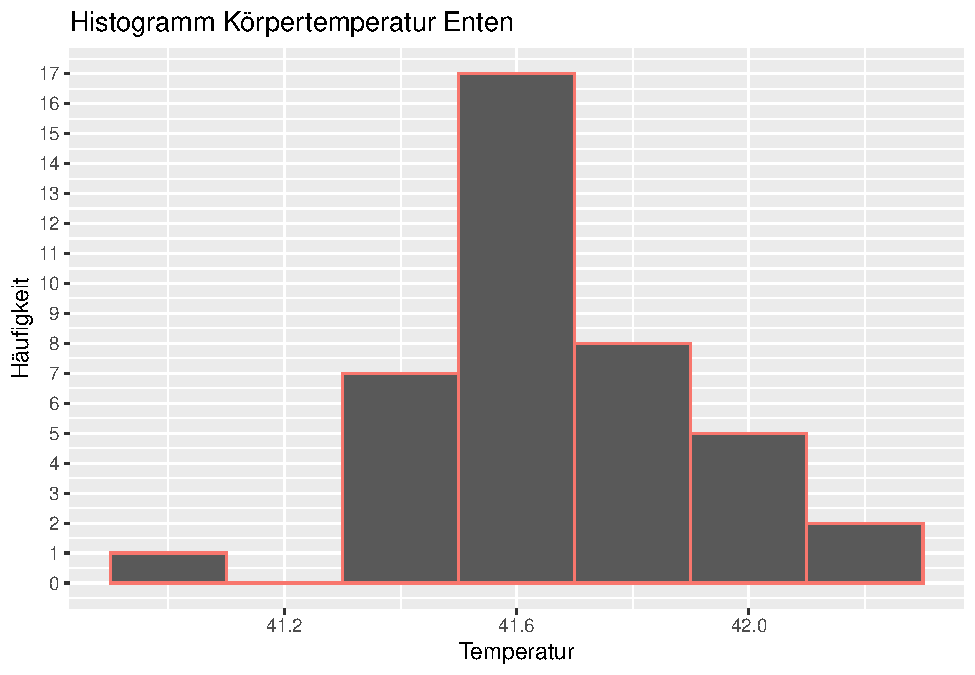
\includegraphics{aps_statistik1_files/figure-latex/enten_histogramm-1.pdf}

Aufgrund dieser Darstellung kann die Veterinärin nun sehen, wie häufig welche Körpertemperaturen sind. Dies wird die \textbf{Verteilung} des Merkmals genannt. Sie bemerkt zum Beispiel, dass Beobachtungen der Körpertemperatur rund um 41.6°C am häufigsten sind und tiefere und höhere Temperaturen seltener vorkommen. Auf einen Blick sieht sie auch, dass die Temperatur aller Enten zwischen 41°C und 42.2°C war.

Die Verteilung eines Merkmals zu kennen ist hilfreich, jedoch in vielen Situationen (z. B. in der Kommunikation) noch zu komplex. Einfacher ist es die Komplexität einer Verteilung auf zwei Faktoren herunterzubrechen: Die Zentralität und die Variabilität eines Merkmals.

\subsection{Zentralität}\label{zentralitaet}

Mit der Zentralität ist ein Wert gemeint, welcher die zentrale Tendenz des Merkmals abbildet. Um die Zentralität zu messen, gibt es drei Möglichkeiten:

\begin{itemize}
\tightlist
\item
  Der \textbf{Modus} ist der am häufigsten vorkommende Wert. Im Beispiel ist das der Wert 41.52, welcher 3 mal und damit am häufigsten vorkommt.
\item
  Wenn die Werte des Merkmals aufsteigend sortiert werden und der Wert betrachtet wird, welcher die Beobachtungen in eine tiefere und eine höhere Hälfte teilt, dann wird dieser Wert als \textbf{Median} (abgekürzt \emph{Mdn}, Symbol \(\tilde{x}\)) bezeichnet. Bei einer geraden Anzahl Beobachtungen, wird in der Regel der Durchschnittswert der beiden mittigsten Beobachtungen verwendet. Im Beispiel haben wir 40 Beobachtungen. Der Median entspricht also dem Durchschnittswert zwischen dem 20. und dem 21. der aufsteigend sortierten Werte 41.07, 41.32, 41.35, 41.43, 41.46, 41.46, 41.48, 41.5, 41.51, 41.52, 41.52, 41.52, 41.53, 41.53, 41.54, 41.58, 41.58, 41.6, 41.62, 41.65, 41.66, 41.67, 41.67, 41.69, 41.7, 41.72, 41.8, 41.81, 41.81, 41.82, 41.82, 41.88, 41.89, 41.92, 41.92, 41.96, 42.01, 42.06, 42.14, 42.18, also 41.655.
\item
  Das \textbf{arithmetische Mittel} (abgekürzt \emph{M}, Symbol \(\bar{x}\)) bezeichnet, was gemeinhin mit Durchschnitt gemeint ist. Wenn wir die erste von insgesamt \(n\) Beobachtung mit \(x_1\) und die letzte Beobachtung mit \(x_n\) bezeichnen, so ist das arithmetische Mittel
\end{itemize}

\begin{equation}
\bar{x} = \frac{1}{n}\sum^n_{i=1} x_i
\label{eq:mean}
\end{equation}

Im Beispiel ist das arithmetische Mittel der Körpertemperaturen 41.6725.

\begin{caution}

\begin{remark}
\emph{Erklärung der Formel}: Hier wird zum ersten Mal eine Formel verwendet. \(\sum\) steht für die Summe von allen Beobachtungen \(x_i\), wenn der Index \(i\) in \(1\)-Schritten von der Zahl unter dem Summenzeichen \(i=1\) bis zu der Zahl oben am Summenzeichen \(i=n\) läuft. In unserem Beispiel ist \(n=40\), also ist \(i = 1, 2, 3, 4, \ldots, 39, 40\). Der Teil \(\sum^n_{i=1} x_i\) bedeutet also nichts anderes als \(x_1 + x_2 + \ldots + x_{39} + x_{40}\), also die Summe aller Beobachtungen. \(\frac{1}{n}\) bedeutet, dass wir diese Summe jetzt noch durch die Anzahl Beobachtungen teilen.

\emph{Welchen Einfluss haben die verschiedenen Einflussgrössen}: Dies wird in Übung \ref{exr:theorie-mdn-mean} erklärt.
\end{remark}

\end{caution}

Jedes dieser Masse für die Zentralität hat Vor- und Nachteile und sie werden dementsprechend in unterschiedlichen Situationen eingesetzt, siehe Übungen.

\subsection{Variabilität}\label{variabilitaet}

TODO: Quantile
TODO: Standardabweichung

\section{Übungen}\label{intervallskaliertes-merkmal-uebungen}

\begin{exercise}
\protect\hypertarget{exr:enten-hist-mean-sd}{}\label{exr:enten-hist-mean-sd}\leavevmode

\begin{enumerate}
\def\labelenumi{(\alph{enumi})}
\tightlist
\item
  Versuch selbst ein Histogramm der Daten oben (\emph{Enten\_n40.sav}) mit Jamovi zu erstellen und begründe, weshalb es nicht gleich aussieht wie das Histogramm oben.
\item
  Berechne zusätzlich das arithmetische Mittel und die Standardabweichung des Merkmals.
\end{enumerate}

\end{exercise}

\begin{solution}
\leavevmode

\begin{figure}
  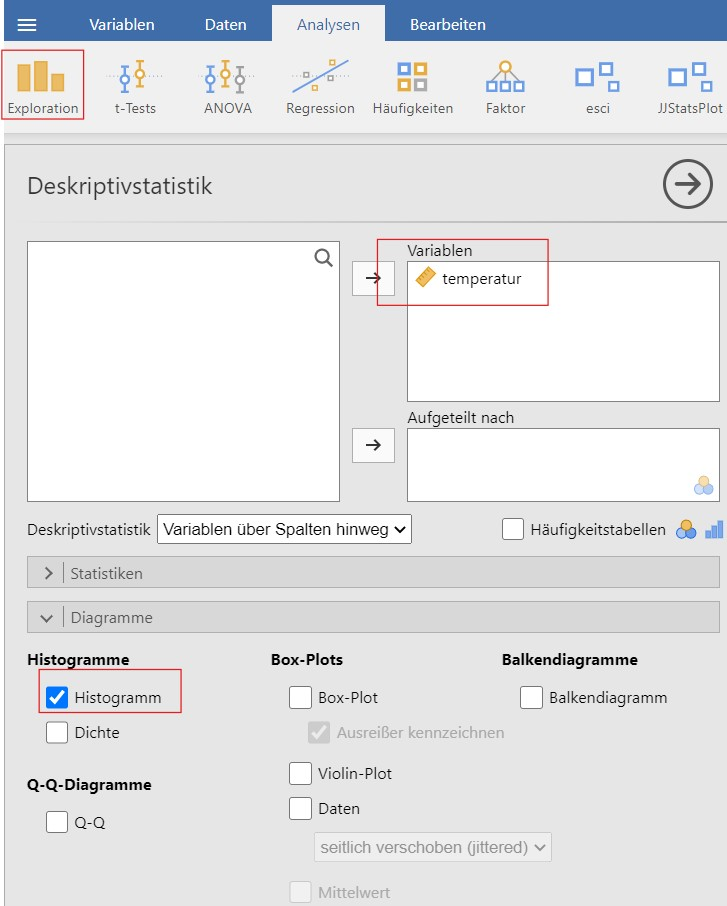
\includegraphics[width=0.5\linewidth]{figures/Enten_n40_instr_histogramm} 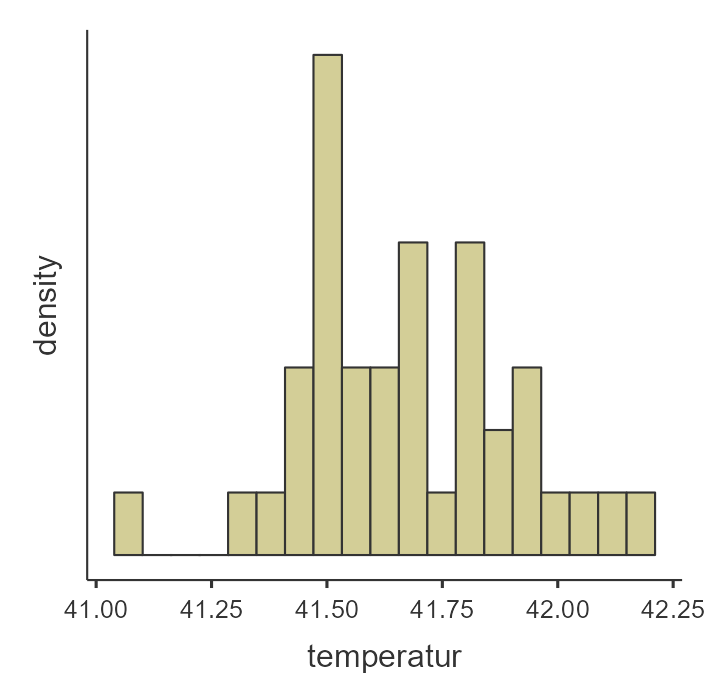
\includegraphics[width=0.5\linewidth]{figures/Enten_n40} \caption{Links: Jamovi-Anleitung zur Erstellung des Histogramms; rechts: Histogramm der Temperatur.}\label{fig:enten-hist-mean-sd}
  \end{figure}

\begin{enumerate}
\def\labelenumi{(\alph{enumi})}
\item
  Das Histogramm, siehe Abbildung \ref{fig:enten-hist-mean-sd} sieht nicht gleich aus, da Jamovi die Temperaturabschnitte kürzer gewählt hat nämlich bei 0.125°C statt 0.2°C wie oben im Text. In Jamovi gibt es aktuell keine Möglichkeit die Abschnittsweite anzupassen. Ein Histogramm sieht immer anders aus je nach ausgewählter Abschnittsweite.
\item
  TODO
\end{enumerate}

\end{solution}

\begin{exercise}
\protect\hypertarget{exr:theorie-mdn-mean}{}\label{exr:theorie-mdn-mean}

In einem psychologischen Test machen \(5\) Probandinnen die Werte \(18, 21, 20, 19, 22\). Um mit einer Zahl zu sagen, wo die Testresultate liegen, wird ein zentraler Wert berechnet.

\begin{enumerate}
\def\labelenumi{(\alph{enumi})}
\tightlist
\item
  Wie gross ist das arithmetische Mittel und der Median dieser Werte?
\item
  Nehme an, der Testleiter hat den Wert der ersten Probandin falsch in seine Tabelle übertragen - statt \(18\) hat er \(81\) geschrieben. Wie gross ist das arithmetische Mittel und der Median dieser Werte in diesem Fall?
\item
  Was sagt dies über den Median und das arithmetische Mittel aus?
\end{enumerate}

\end{exercise}

\begin{solution}

Die Aufgabe kann im Kopf gelöst werden, oder mithilfe eines Taschenrechners, oder indem die Zahlen manuell bei Jamovi eingegeben werden.

\begin{enumerate}
\def\labelenumi{(\alph{enumi})}
\tightlist
\item
  Wir haben hier \(n=5\) Beobachtungen, nämlich \(x_1 = 18, x_2 = 21, x_3 = 20, x_4 = 19, x_5=22\). Wird dies in die Formel \eqref{eq:mean} eingesetzt, so gibt dies das arithmetische Mittel
  \[\bar{x} = \frac{1}{n}\sum^n_{i=1} x_i = \frac{1}{n}(x_1 + x_2 + x_3 + x_4 + x_5) =  \frac{1}{5}(18+ 21+ 20+ 19+ 22) = 20.\]
  Um den Median zu berechnen, werden die Werte zuerst aufsteigend sortiert \(18, 19, 20, 21, 22\). Der Wert, welcher die Werte in eine grössere und eine kleinere Hälfte teilt, ist hier \(20\), was dem Median entspricht.
\item
  Die Beobachtungen sind jetzt \(x_1 = 81, x_2 = 21, x_3 = 20, x_4 = 19, x_5=22\). Analog wie in (a) kann demnach das arithmetische Mittel als \(\bar{x} = 32.6\) bestimmt werden. Die aufsteigend sortierten Beobachtungen sind nun \(19, 20, 21, 22, 81\). Der Median ist also \(21\).
\item
  Durch die fälschliche Übertragung eines Wertes, ist das arithmetische Mittel sehr stark und der Median fast gar nicht beeinflusst worden. Wenn die Daten wenige fehlerhafte Beobachtungen enthalten, ist der Median das bessere Mass für den zentralen Wert als das arithmetische Mittel. Wenn die Daten keine Fehler enthalten, ist das arithmetische Mittel gleich gut geeignet wie der Median.
\end{enumerate}

\end{solution}

\chapter{Stichprobenziehung}\label{stichprobenziehung}

Forschende haben ein Messinstrument für Angst entwickelt, welches STAI (State-Trait Anxiety Inentory) \citep{spielberger1983manual}. Sie erheben dabei unter anderem einen Wert zwischen \(20\) und \(80\) für eine Zustandsangst. A priori haben die Forschenden keine Ahnung, wie ängstlich eine Person im Durchschnitt ist oder ob die ganze Skala der Werte genutzt wird. Die Forschenden machen deshalb eine kleine Befragung mit \(30\) zufällig ausgewählten Studierenden. Zufällig ausgewählte Beobachtungen eines Merkmals werden als \textbf{Stichprobe} bezeichnet. Die Forschenden finden die zusammenfassenden Werte \(M=43.2, s = 7.8, n = 30\) für die Zustandsangst in ihrer Stichprobe.

Anschliessend stellt sich die Frage, wie stark diese Werte basierend auf dieser Stichprobe Zustandsangst von allen Personen widerspiegelt. Alle Personen oder generell alle möglichen Beobachtungen eines Merkmals, werden als \textbf{Population} oder \textbf{Grundgesamtheit} bezeichnet. Eine Stichprobe ist für viele Analyseverfahren repräsentativ für eine Population, wenn sie zufällig aus dieser Population gezogen. Ist dies gegeben, wird die Stichprobe auch als \textbf{Zufallsstichprobe} bezeichnet.

\begin{remark}
Viele Studien basieren auf Testresultaten von Studierenden, weil diese nahe am Forschungsbetrieb sind und damit über Studien informiert sind oder für wenig Geld oder Bildungsanerkennung an Studien teilnehmen. Einige dieser Studien generalisieren ihre Forschungsresultate nachher auf alle Personen. Dies ist in der Regel falsch, da Studierende nicht repräsentativ für die Gesamtbevölkerung sind (Altersstruktur, Geschlechtsverteilung, Vermögen, usw.). Die Frage, wie eine repräsentative Stichprobe würde den Rahmen dieses Buches sprengen.
\end{remark}

\section{Was ist das Problem der Stichprobenziehung?}\label{stichprobenziehung-problem}

Es wird angenommen, dass sich alle Personen der Population in einem Zimmer befinden. In Abbildung \ref{fig:srs-intervall-nocol} ist dieses Zimmer aus der Vogelperspektive dargestellt, wobei jeder Punkt im schwarzen Kasten einer Person der Population. Die Personen im Zimmer, respektive die Beobachtungen in der Population sind normalerweise nicht sichtbar. Aus diesem Zimmer wurden also 30 Personen geholt und befragt also sichtbar gemacht, was der Zufallsstichprobe entspricht. Die Zufallsstichprobe ist gekennzeichnet durch die Punkte über dem Zimmer, oberhalb des Pfeils. Die Farben der Punkte sind jetzt bekannt und entsprechen der jeweiligen Zustandesangst der beobachteten Personen.

\begin{figure}
\centering
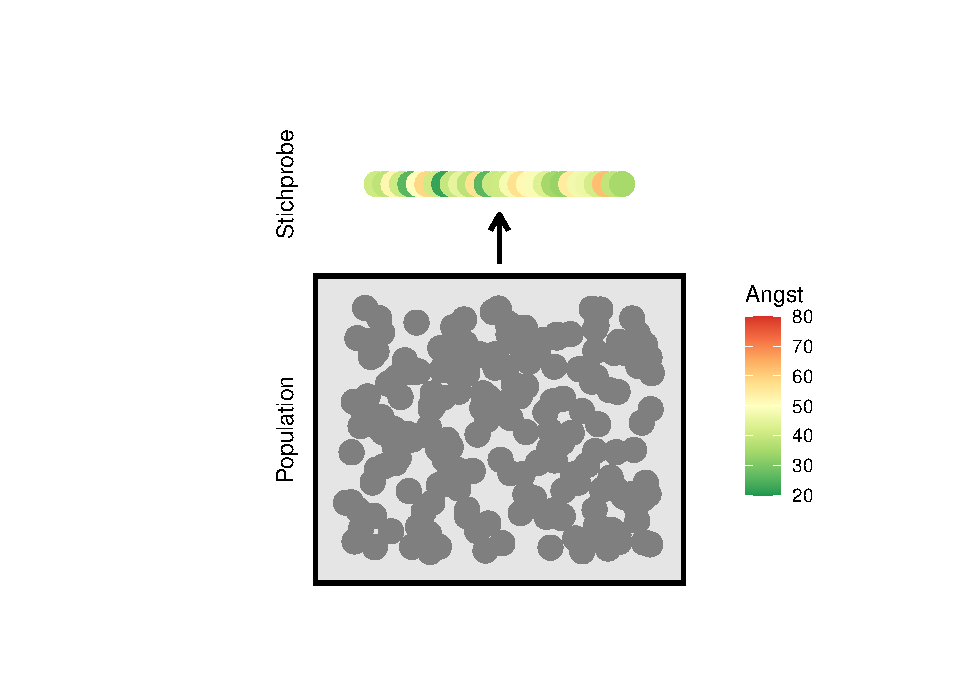
\includegraphics{aps_statistik1_files/figure-latex/srs-intervall-nocol-1.pdf}
\caption{\label{fig:srs-intervall-nocol}Population mit unbekannter Zustandsangst.}
\end{figure}

Da die Stichprobe nun eben zufällig gezogen wurde, das heisst zufällig Personen aus dem Zimmer geholt wurden, kann es nun sein, dass die Stichprobe einer Population wie in Abbildung \ref{fig:srs-intervall-high-p} entstammt.

\begin{figure}
\centering
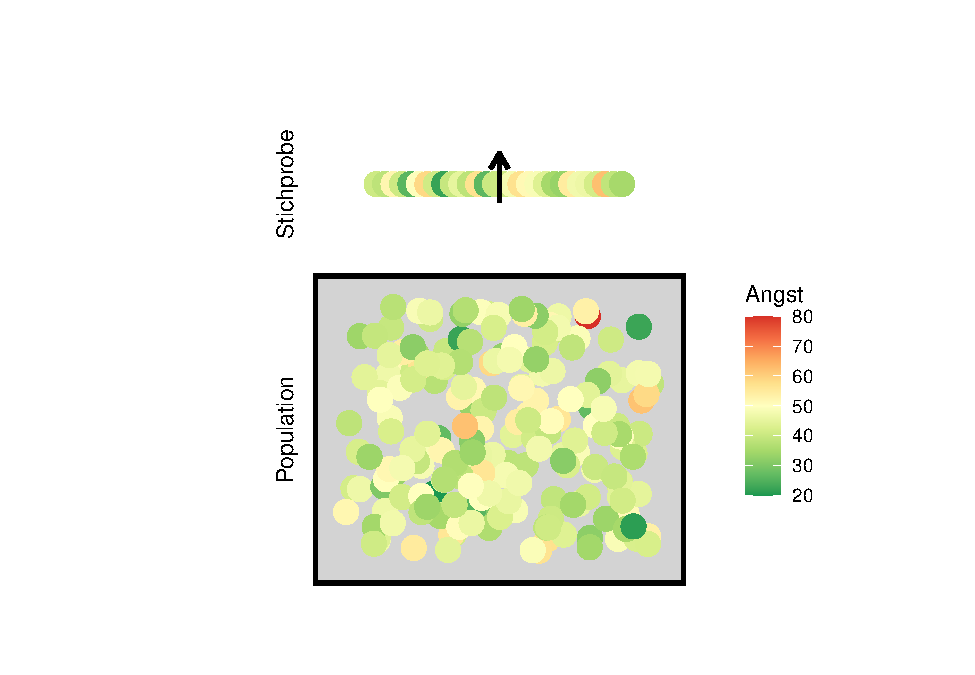
\includegraphics{aps_statistik1_files/figure-latex/srs-intervall-high-p-1.pdf}
\caption{\label{fig:srs-intervall-high-p}Population mit ähnlichen Zustandsangst-Werten wie in der Stichprobe.}
\end{figure}

Es könnte aber auch sein, dass die Stichprobe einer Population mit viel höherer Zusatandsangst, wie in Abbildung \ref{fig:srs-intervall-low-p} dargestellt, entstammt. Dies wird zwar weniger häufig vorkommen als der Fall oben, aber ist trotzdem möglich.

\begin{figure}
\centering
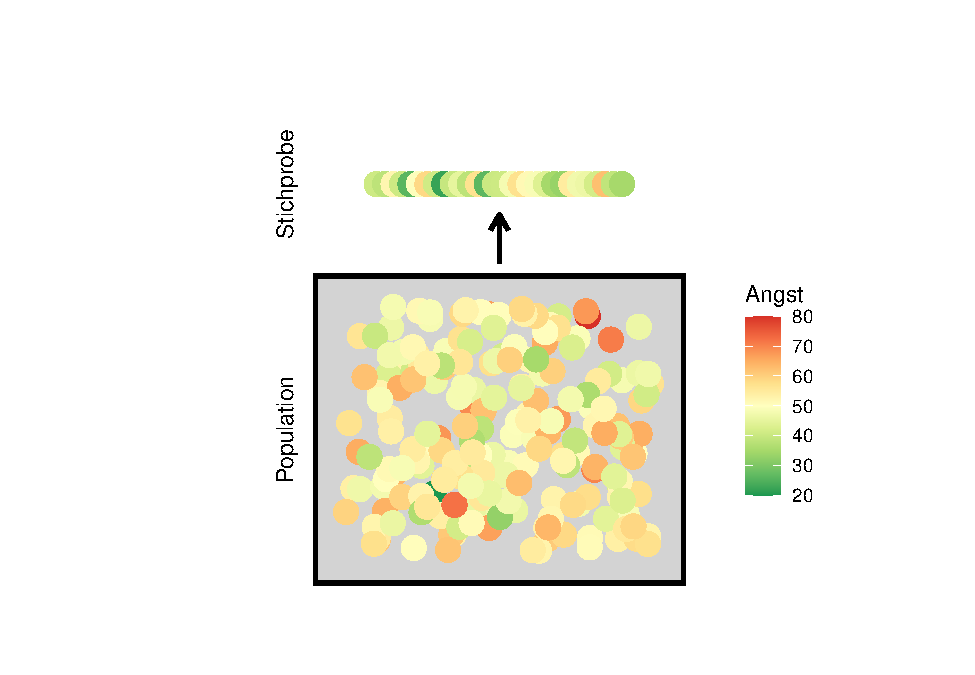
\includegraphics{aps_statistik1_files/figure-latex/srs-intervall-low-p-1.pdf}
\caption{\label{fig:srs-intervall-low-p}Population mit höheren Zustandsangst-Werten als in der Stichprobe.}
\end{figure}

Das Problem der zufälligen Stichprobenziehung ist also, dass nie ganz klar ist, wie die darunterliegende Population aussieht. Sind die Werte der Stichprobe tief, weil zufällig gerade Studierende mit tiefer Zustandsangst beobachtet wurden, oder haben tatsächlich die meisten Studierenden eine tiefe Zustandsangst?

\section{Wie kann man Aussagen über die Grundgesamtheit machen?}\label{stichprobenziehung-luxf6sung}

Die Lösung dieses Problems funktioniert intuitiv wie folgt: Man stellt sich vor, die Stichprobenziehung würde erneut gemacht, und dann nochmal und dann nochmal. So oft, bis man einen guten Eindruck davon hat, wie häufig eine Stichprobe mit eher tiefen Zustandsangst-Werten wie bei der Stichprobe im Beispiel vorkommt. Im Szenario, in welchem in der Population tatsächlich tiefe Werte häufig vorkommen, kann dies aussehen wie in Abbildung \ref{fig:srs-intervall-high-p-many}. Stichproben mit eher tiefen Zustandsangst-Werten kommen hier häufig vor.

\begin{figure}
\centering
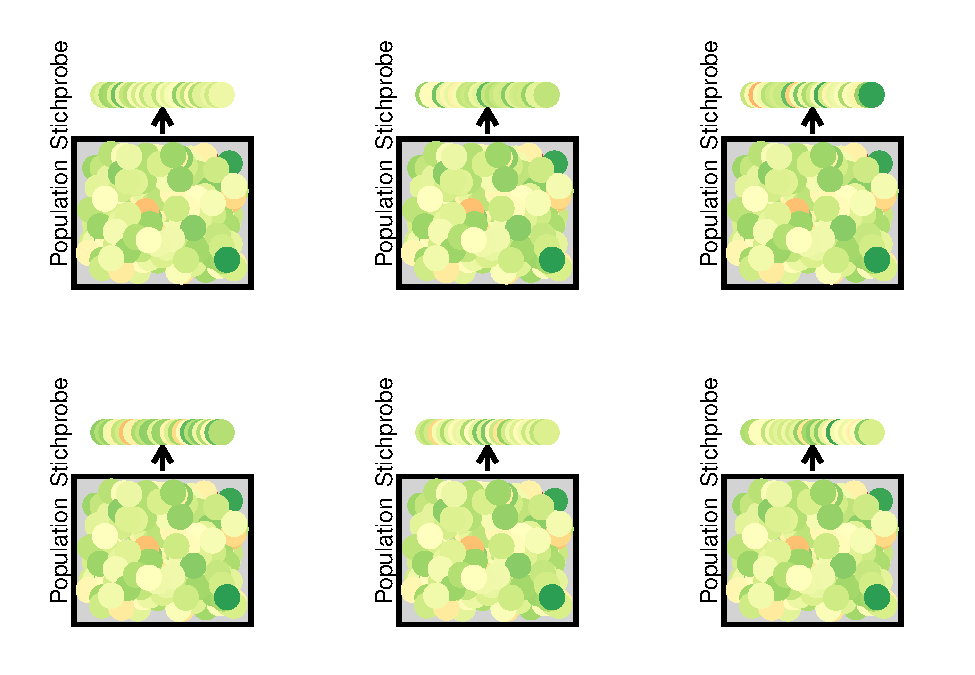
\includegraphics{aps_statistik1_files/figure-latex/srs-intervall-high-p-many-1.pdf}
\caption{\label{fig:srs-intervall-high-p-many}TODO.}
\end{figure}

Im Szenario, in welchem in der Population tatsächlich höhere Werte häufig vorkommen, kann dies aussehen wie in Abbildung \ref{fig:srs-intervall-low-p-many}. Stichproben mit eher tiefen Zustandsangst-Werten kommen hier selten oder gar nicht vor.

\begin{figure}
\centering
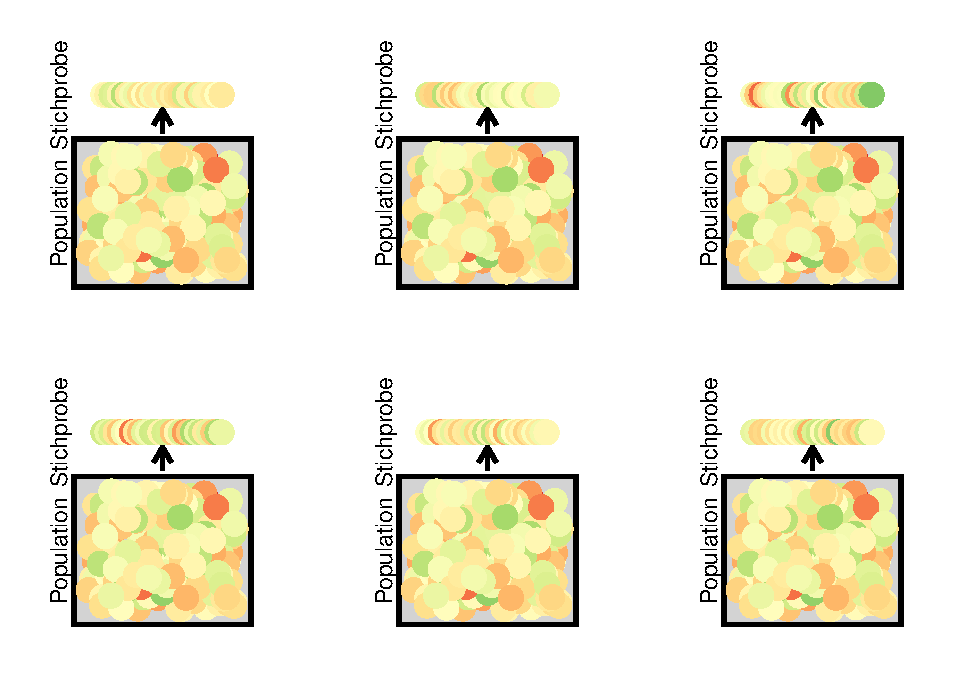
\includegraphics{aps_statistik1_files/figure-latex/srs-intervall-low-p-many-1.pdf}
\caption{\label{fig:srs-intervall-low-p-many}TODO.}
\end{figure}

Es kann also zusammenfassend gesagt werden, dass die gezogene Stichprobe wohl eher aus einer Population mit tiefen Zustandsangst-Werten gezogen wurde als aus einer Population mit eher höheren Zustandsangst-Werten. Ganz sicher kann man jedoch nie sein, da die Werte in der Population eigentlich unbekannt sind. Eine genaue Quantifizierung dieser Unsicherheit kann mit Hilfe der Statistik erreicht werden und wird in den folgenden Kapiteln dieses Buches erläutert.

\section{Übungen}\label{uxfcbungen}

\chapter{Durchschnitt und Standardabweichung schätzen}\label{durchschnitt-und-standardabweichung-schuxe4tzen}

Wie die in Abschnitt @ref(stichprobenziehung-lösung) erklärte Lösung für das Problem der zufälligen Stichprobe konkret gemacht werden muss hängt von der Problemstellung ab.

\section{Wo liegt der Durchschnitt der Grundgesamtheit?}\label{wo-liegt-der-durchschnitt-der-grundgesamtheit}

Ein Parameter über welchen wir gerne eine Aussage treffen würden ist die zentrale Tendenz in der Grundgesamtheit. Diese wird \textbf{Erwartungswert} (Symbol \(\mu\) {[}gr.: mü{]}) genannt. Wenn das arithmetische Mittel der Stichprobe berechnet wird, ergibt dies auch ein Schätzwert für besagten Erwartungswert. Aufgrund der zufälligen Stichprobenziehung ist jedoch auch klar, dass dieser Schätzwert nie genau dem wahren Erwartungswert entspricht.

Die Folgefrage ist also wie genau unsere Schätzung ist. Um dies zu quantifizieren, wiederholen wir die Stichprobenziehung und berechnen das arithmetische Mittel dieser zweiten Stichprobe. Dann wiederholen wir diesen Prozess, zum Beispiel 1000 mal.

\begin{figure}
\centering
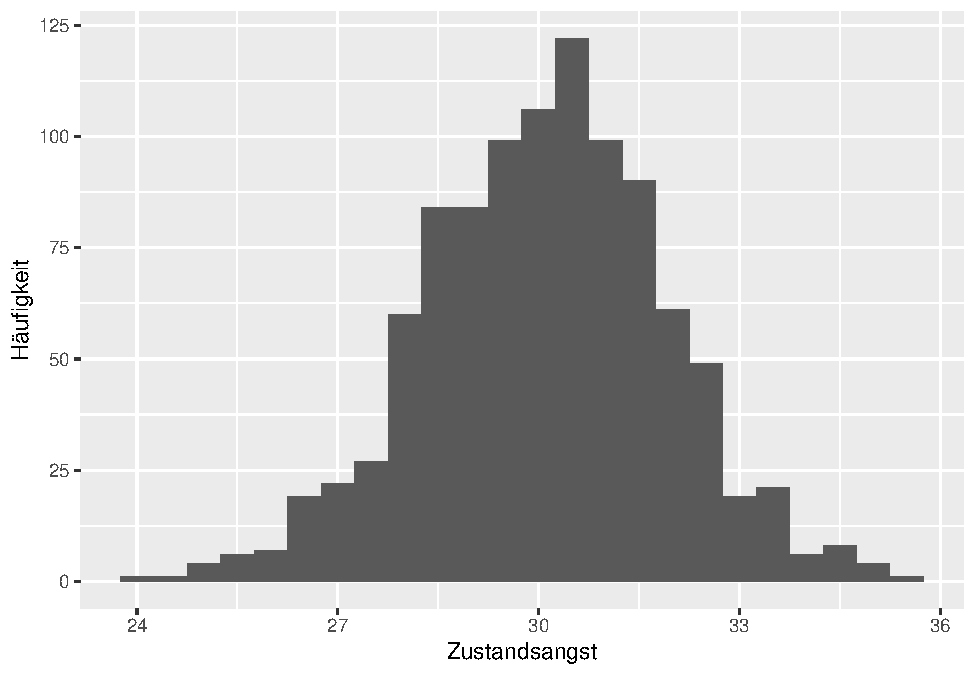
\includegraphics{aps_statistik1_files/figure-latex/hist-mean-estimation-1.pdf}
\caption{\label{fig:hist-mean-estimation}Verteilung der arithmetischen Mittel von 1000 zufällig gezogenen Stichproben der Zustandsangst.}
\end{figure}

Die Häufigkeitsverteilung der berechneten arithmetischen Mittelin Abbildung \ref{fig:hist-mean-estimation} lässt nun Aussage über die Häufigkeit und damit über die Wahrscheinlichkeit von gewissen Werten als Erwartungswert zu. Ein Durchschnittswert der Zustandesangst um die 30 ist hier am wahrscheinlichsten und ein Wert tiefer als 27 oder höher 33 eher selten. Um diese Schätzung wissenschaftlicher präziser zu gestalten, werden konventionell die 95\% häufigsten Werte (die höchsten Balken im Histogramm) als wahrscheinlich betrachtet. Die 5\% verbleibenden Werte, verteilt auf das untere und obere Extrem, werden als unwahrscheinlich betrachtet. Das 2.5\% Perzentil trennt die 2.5\% tiefsten arithmetischen Mittel ab und liegt im Beispiel bei 26.5. Das 97.5.5\%-Perzentil trennt die höchsten 2.5\% (oder eben die tiefsten 97.5\%) arthmetischen Mittel ab und liegt bei 33.6.

\begin{figure}
\centering
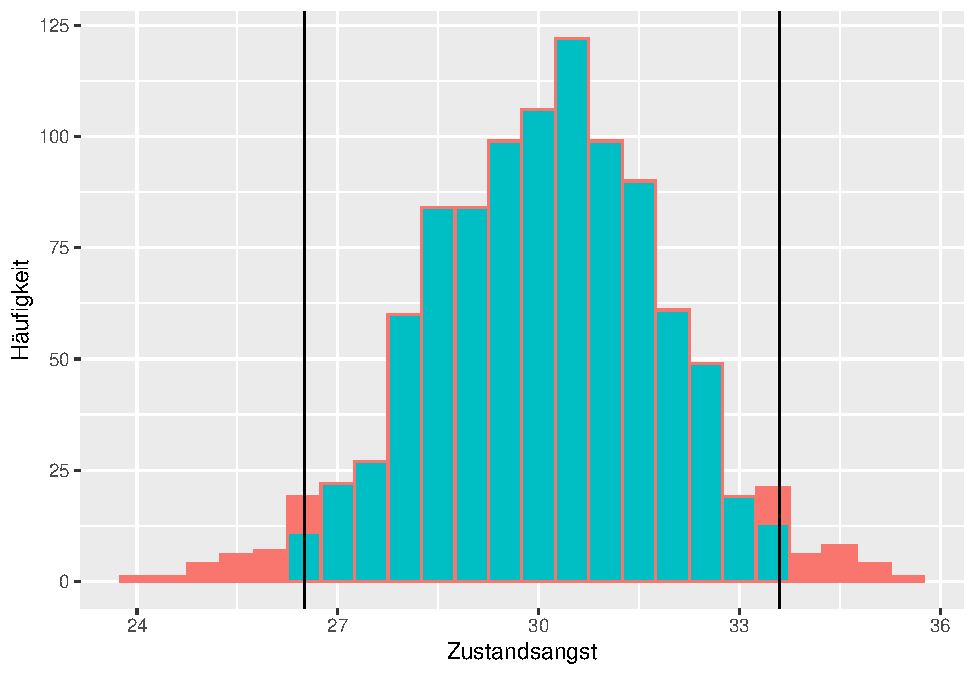
\includegraphics{aps_statistik1_files/figure-latex/hist-mean-estimation1-1.pdf}
\caption{\label{fig:hist-mean-estimation1}Verteilung der arithmetischen Mittel von 1000 zufällig gezogenen Stichproben der Zustandsangst.}
\end{figure}

TODO: explain example 2 likert scale

\begin{verbatim}
## Warning: Removed 4 rows containing missing values or values outside the scale range
## (`geom_bar()`).
\end{verbatim}

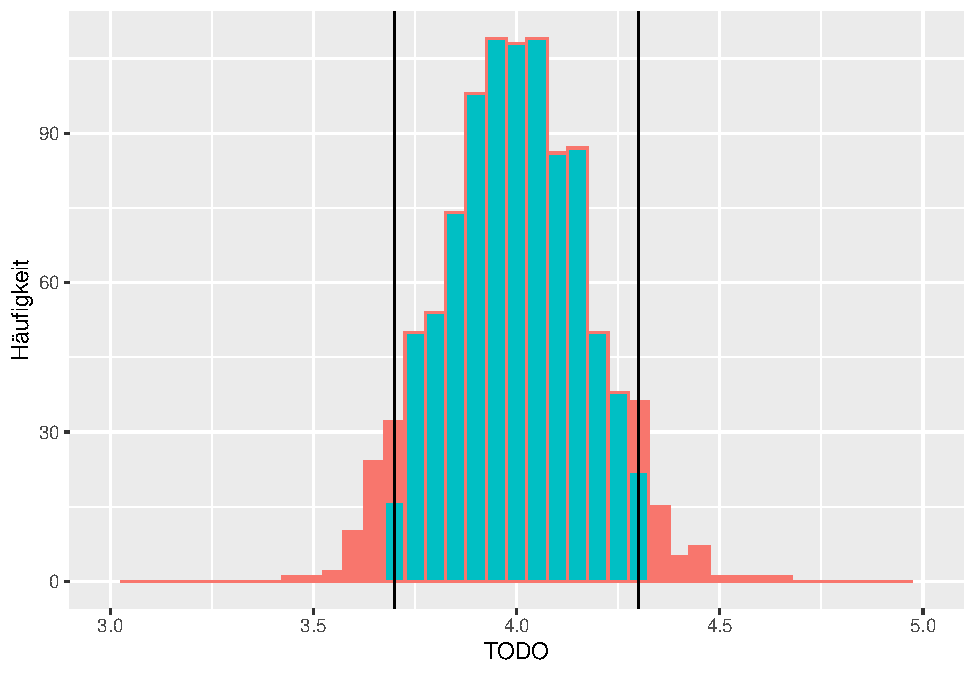
\includegraphics{aps_statistik1_files/figure-latex/hist-mean-estimation2-1.pdf}
TODO: explain quantiles.

Das Problem mit diesem Vorgehen ist, dass es aus finanziellen oder technischen Gründen selten möglich ist mehrere Stichproben aus derselben Population zu ziehen. Glücklicherweise haben Statistiker:innen herausgefunden, dass die Häufigkeitsverteilungen wie in Abbildungen \ref{fig:hist-mean-estimation1} und \ref{fig:hist-mean-estimation2} immer dieselbe Verteilung haben und dies unabhängig davon wie die ursprüngliche Verteilung des Merkmals aussah. Diese Verteilung ist eine sogenannte \textbf{Normalverteilung}.

Die Normalverteilung sieht eine Glocke ähnlich. Deshalb wird sie auch Gausssche Glockenkurve nach Carl F. Gauss (1777-1855) benannt. Die Normalverteilung kann mit nur zwei Parametern beschrieben werden.

\begin{itemize}
\tightlist
\item
  \(\mu_g\) gibt an, wo auf der x-Achse der höchste Punkt der Glocke liegt
\item
  \(\sigma_g\) gibt an, wie flach die Glockenform ist (ein grosser Wert entspricht einer flachen Glockenform, ein tiefer Wert einer steilen Glockenform).
\end{itemize}

Auf \href{https://seeing-theory.brown.edu/probability-distributions/index.html\#section2}{seeing-theory.brown.edu \textgreater{} Continuous \textgreater{} Normal} kann der Einfluss von \(\mu\) und \(\sigma\) auf die Normalverteilung erfahren werden.

Diese Tatsache, dass die Durchschnitte aller Merkmale normalverteilt sind, ist so zentral für die Statistik, dass sie \textbf{Zentraler Grenzwertsatz} genannt wurde. Der zentrale Grenzwertsatz besagt geneauer, dass bei einem Merkmal mit Erwartungswert \(\mu\) und Standardabweichung \(\sigma\), der Durchschnitt aller Stichprobenwerte einer Normalverteilung mit \(\mu_g = \mu\) und \(\sigma_g = \frac{\sigma}{\sqrt{n}}\) entspricht, wobei \(n\) die Stichprobengrösse bezeichnet.

\begin{remark}
\leavevmode

\begin{itemize}
\tightlist
\item
  \(\mu_g = \mu\) bedeutet, dass der Wert, welcher unter der normalverteilung am wahrscheinlichsten ist, genau dem Erwartungswert des untersuchten Merkmales entspricht.
\item
  \(\sigma_g = \frac{\sigma}{\sqrt{n}}\) hat zwei Implikationen:

  \begin{itemize}
  \tightlist
  \item
    je grösser die Streuung des Merkmals (grosses \(\sigma\)) desto breiter ist auch die Streuung der arithmetischen Mittel (grosses \(\sigma_g\)). Dies bedeutet, je weniger Streuung das Merkmal aufweist, desto genauer ist die Bestimmung des Erwartungswertes des Merkmales.
  \item
    je grösser die Anzahl Beobachtungen \(n\), desto kleiner die Streuung der arithmetischen Mittel (kleines \(\sigma_g\)). Dies bedeutet, je grösser die Stichprobe ist, desto genauer ist die Bestimmung des Erwartungswertes des Merkmales.
  \end{itemize}
\end{itemize}

\end{remark}

Die Abbildungen \ref{fig:normal-approx} und \ref{fig:normal-approx1} illustrieren den zentralen Grenzwertsatz für Beispiel 1 und 2 respektive. Dabei wird einstweilen angenommen, dass \(\mu\) und \(\sigma\) bekannt sind. Diese Annahme wird später aufgelöst und dient hier lediglich der Illustration.

\begin{figure}
\centering
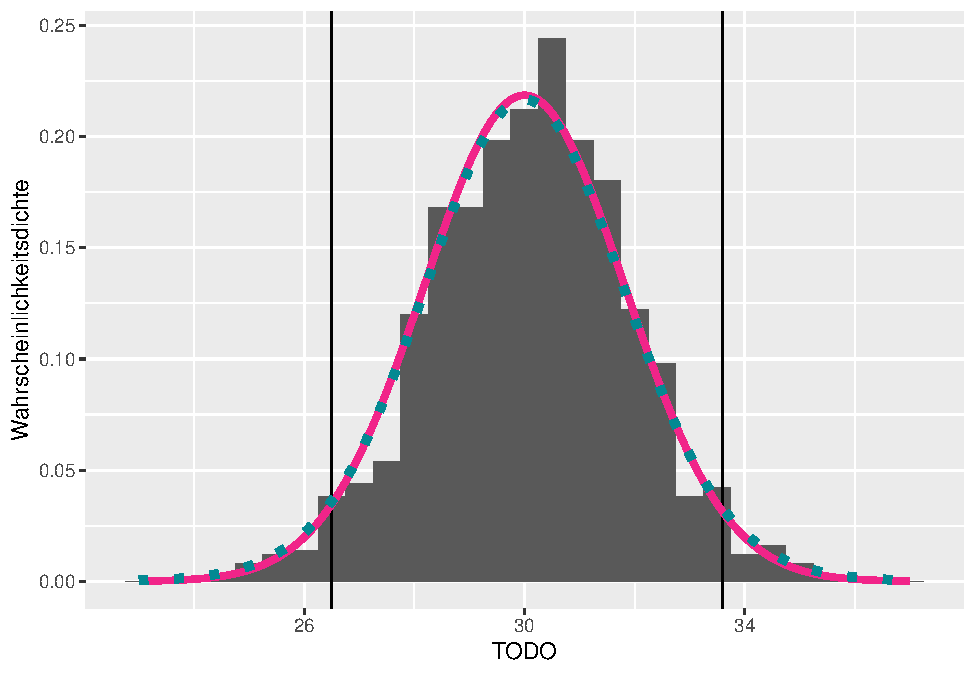
\includegraphics{aps_statistik1_files/figure-latex/normal-approx-1.pdf}
\caption{\label{fig:normal-approx}Die arithmetischen Mittel sind Normalverteilt mit Parametern \(\mu_g = 30\) und \(\sigma_g = 10 / \sqrt{30}\).}
\end{figure}

\begin{figure}
\centering
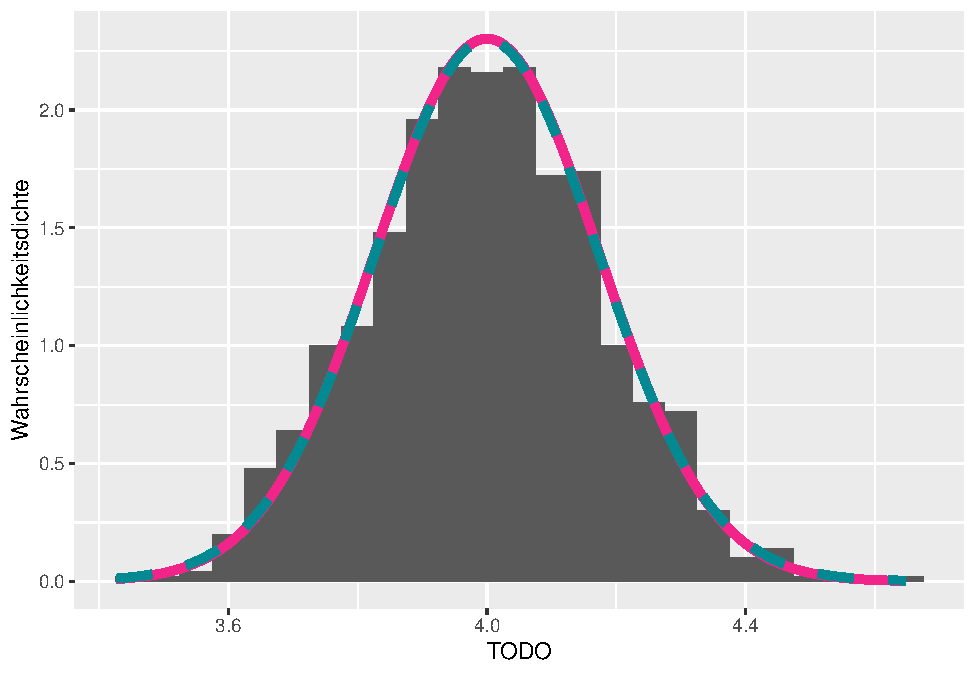
\includegraphics{aps_statistik1_files/figure-latex/normal-approx1-1.pdf}
\caption{\label{fig:normal-approx1}Die arithmetischen Mittel sind Normalverteilt mit Parametern \(\mu_g = 4\) und \(\sigma_g = 1.73 / \sqrt{100}\).}
\end{figure}

Die Erkenntnis des zentralen Grenzwertsatz macht also das wiederholte ziehen von Stichproben unnötig. Die Normalverteilung ist theoretisch konstruiert und ihr 2.5\%- und 97.5\%-Perzentil können theoretisch hergeleitet werden. Tabelle \ref{tab:quantiles-norm} wird kann beobachtet werden, dass für unsere zwei Beispiele die Perzentile der Stichprobe und der Normalverteilung sehr ähnlich, wenn auch nicht exakt gleich sind. Die Ungenauigkeit rührt daher, dass der zentrale Grenzwertsatz nur dann exakt funktioniert, wenn die Anzahl Beobachtungen (unendlich) gross ist.

\begin{table}

\caption{\label{tab:quantiles-norm}Vergleich Perzentile der Stichprobe und der theoretischen Verteilung.}
\centering
\begin{tabular}[t]{r|r|r|r|r}
\hline
Beispiel & 2.5\%-Perzentil (Stichprobe) & 97.5\%-Perzentil (Stichprobe) & 2.5\%-Perzentil (Normalverteilung) & 97.5\%-Perzentil (Normalverteilung)\\
\hline
1 & 26.5 & 33.6 & 26.421612 & 33.578388\\
\hline
2 & 3.7 & 4.3 & 3.660524 & 4.339476\\
\hline
\end{tabular}
\end{table}

Einstweilen wurde hier angenommen, dass die Streuung des Merkmals \(\sigma\) bekannt ist. Dies ist in der Realität nie der Fall. Wenn \(\sigma\) also auch aus der Stichprobe geschätzt werden muss, ist die Verteilung der arthmetischen Mittel

\[ \bar{x} - \frac{\sigma}{\sqrt{n}} \cdot z_{2.5\%} < \mu < \bar{x} - \frac{\sigma}{\sqrt{n}} \cdot z_{2.5\%}\]

\section{Wo liegt der Durchschnitt der Standardabweichung?}\label{wo-liegt-der-durchschnitt-der-standardabweichung}

\section{Übungen}\label{uxfcbungen-1}

\chapter{Durchschnitt testen}\label{durchschnitt-testen}

\section{Entspricht der Durchschnitt der Grundgesamtheit einem gewissen Wert?}\label{entspricht-der-durchschnitt-der-grundgesamtheit-einem-gewissen-wert}

\section{Weicht der gefundene Durchschnitt stark vom hypothetischen Wert ab?}\label{weicht-der-gefundene-durchschnitt-stark-vom-hypothetischen-wert-ab}

\section{Übungen}\label{uxfcbungen-2}

\part{Gruppenvergleich einer intervallskalierten Variable}\label{part-gruppenvergleich-einer-intervallskalierten-variable}

\chapter{Gruppenvergleich einer intervallskalierten Variable}\label{gruppenvergleich-einer-intervallskalierten-variable}

\section{Zwei Gruppen vergleichen}\label{zwei-gruppen-vergleichen}

\section{Was ist das Problem der Stichprobenziehung?}\label{was-ist-das-problem-der-stichprobenziehung}

\section{Wie kann man Aussagen über die Grundgesamtheit machen?}\label{wie-kann-man-aussagen-uxfcber-die-grundgesamtheit-machen}

\section{Übungen}\label{uxfcbungen-3}

\chapter{Welch-Test}\label{welch-test}

\section{Zwei Gruppen vergleichen}\label{zwei-gruppen-vergleichen-1}

\section{Sind die Durchschnitte der beiden Gruppen in der Grundgesamtheit gleich?}\label{sind-die-durchschnitte-der-beiden-gruppen-in-der-grundgesamtheit-gleich}

\section{Wie stark unterscheiden sich die Durchschnitte?}\label{wie-stark-unterscheiden-sich-die-durchschnitte}

\section{Übungen}\label{uxfcbungen-4}

\chapter*{Begriffsverzeichnis}\label{begriffsverzeichnis}
\addcontentsline{toc}{chapter}{Begriffsverzeichnis}

\begin{itemize}
\tightlist
\item
  \textbf{intervallskaliert}
\item
  \hyperref[NA]{\textbf{arithmetische Mittel}}
\item
  \hyperref[NA]{\textbf{deskriptive Statistik}}
\item
  \textbf{Grundgesamtheit}
\item
  \hyperref[NA]{\textbf{Histogramm}}
\item
  \hyperref[NA]{\textbf{Konfidenzintervalle}}
\item
  \hyperref[NA]{\textbf{Median}}
\item
  \hyperref[NA]{\textbf{Modus}}
\item
  \textbf{Population}
\item
  \textbf{Stichprobe}
\item
  \hyperref[NA]{\textbf{Verteilung}}
\item
  \hyperref[NA]{\textbf{Wahrscheinlichkeitslehre}}
\item
  \textbf{Zufallsstichprobe}
\end{itemize}

  \bibliography{book.bib,packages.bib}

\end{document}
